\documentclass[11pt]{article}
\usepackage{amsmath,amssymb}
\usepackage{graphicx}
\usepackage[margin=1in]{geometry}
\title{Extremal Selection as an Operational Substitute for Coexponentials:\\ Fisher-Controlled Factorization}
\author{Draft}
\date{\today}
\begin{document}
\maketitle
\begin{abstract}
In $\mathbf{Set}$, a coexponential (left adjoint to coproduct) does not exist in general.
We use extremal selection on compact polytopes, componentwise probes, and Fisher off-diagonal leakage $\varepsilon$ to certify when separable optimization is near-optimal.
We give vertex localization, a bound $\Phi(\varepsilon)$, and a constructive vertex algorithm, with reproducible experiments.
\end{abstract}

\section{Introduction}
Categorical duality suggests a coexponential $\dashv$ coproduct dual to curry $\dashv$ product.
Cardinality obstructs a representing object in $\mathbf{Set}$.
We propose an operational substitute: search $\mathrm{ext}(H)$, build block probes, and bound cross-block coupling by $\varepsilon=\|F_{AB}\|_F/\|F_{\mathrm{diag}}\|_F$.

\section{Main results}
\textbf{Theorem 1 (Vertex localization).}
On a compact box $H$, if $C(\theta)=g(\theta_A)+h(\theta_B)+r(\theta)$ with separate monotonicity and axis quasiconvexity, then $\theta^\star\in\mathrm{ext}(H)$.

\textbf{Theorem 2 (Near-optimality).}
$C(\theta^\star)-C(\theta_{\mathrm{sep}})\le \Phi(\varepsilon)$ with
$\Phi(\varepsilon)=\tfrac12 \varepsilon^2 \lambda_{\min}^{-1}\|\theta^\star\|^2\|F_{\mathrm{diag}}\|_F$.

\textbf{Theorem 3 (Constructive probe).}
A componentwise top-$k$ vertex probe attains near-optimality with certificate $\Phi(\varepsilon)$ when $\varepsilon\le\varepsilon_0$.

\section{Experiments}
See auto-generated tables in \texttt{docs/EXPERIMENT\_REPORT.md}.
\begin{figure}[h]
\centering
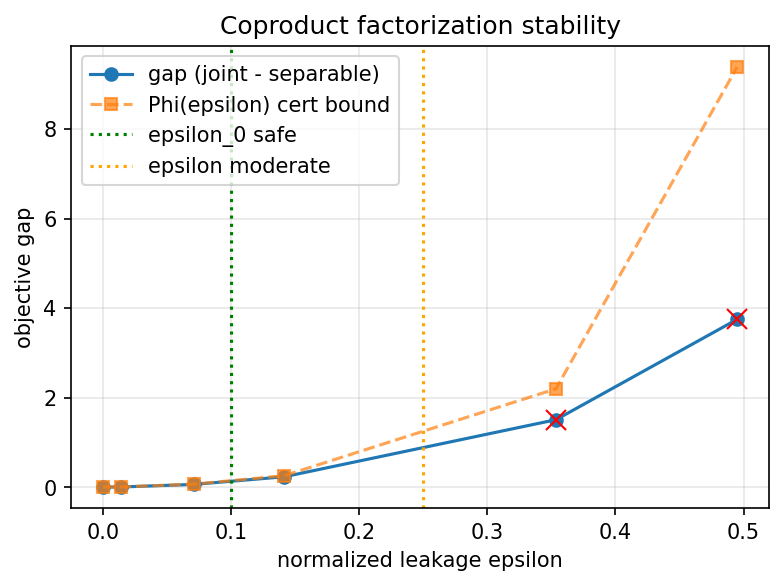
\includegraphics[width=0.75\linewidth]{../experiments/figures/gap_vs_epsilon.png}
\caption{Objective gap vs.\ normalized leakage $\varepsilon$ (quadratic toy).}
\end{figure}
\begin{figure}[h]
\centering
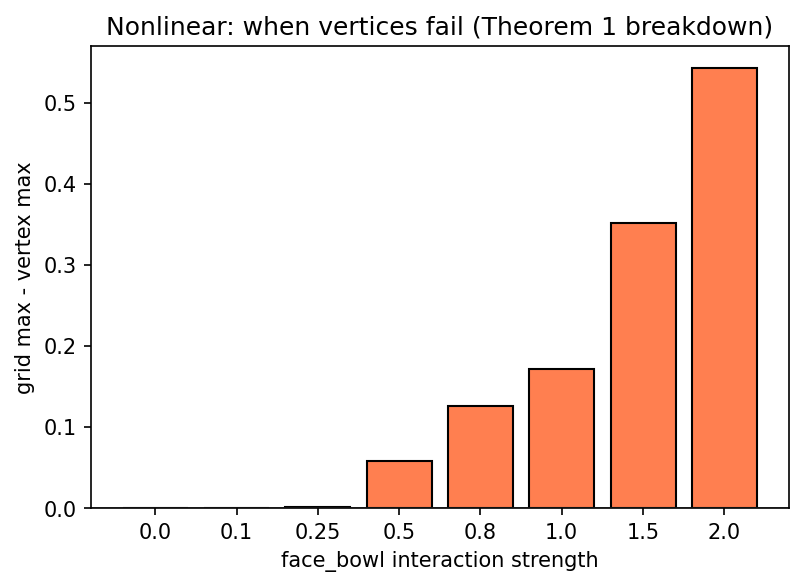
\includegraphics[width=0.75\linewidth]{../experiments/figures/nonlinear_face_bowl.png}
\caption{\texttt{face\_bowl}: grid max minus vertex max (localization breakdown).}
\end{figure}

\section{Conclusion}
Fisher-controlled extremal probes replace absent coexponentials with certifiable, implementable factorization when $\varepsilon$ is small.

\end{document}
